% Appendix Template

\chapter{More Statistical Analysis Results} % Main appendix title

\label{Appendix B} % Change X to a consecutive letter; for referencing this appendix elsewhere, use \ref{AppendixX}

We also derived some statistical result from our processed data. This results is not related to our classifier.
Some of the results are discussed below 
\section{Department wise Different Grade Comparison}

\begin{figure}[H]
   \centering
  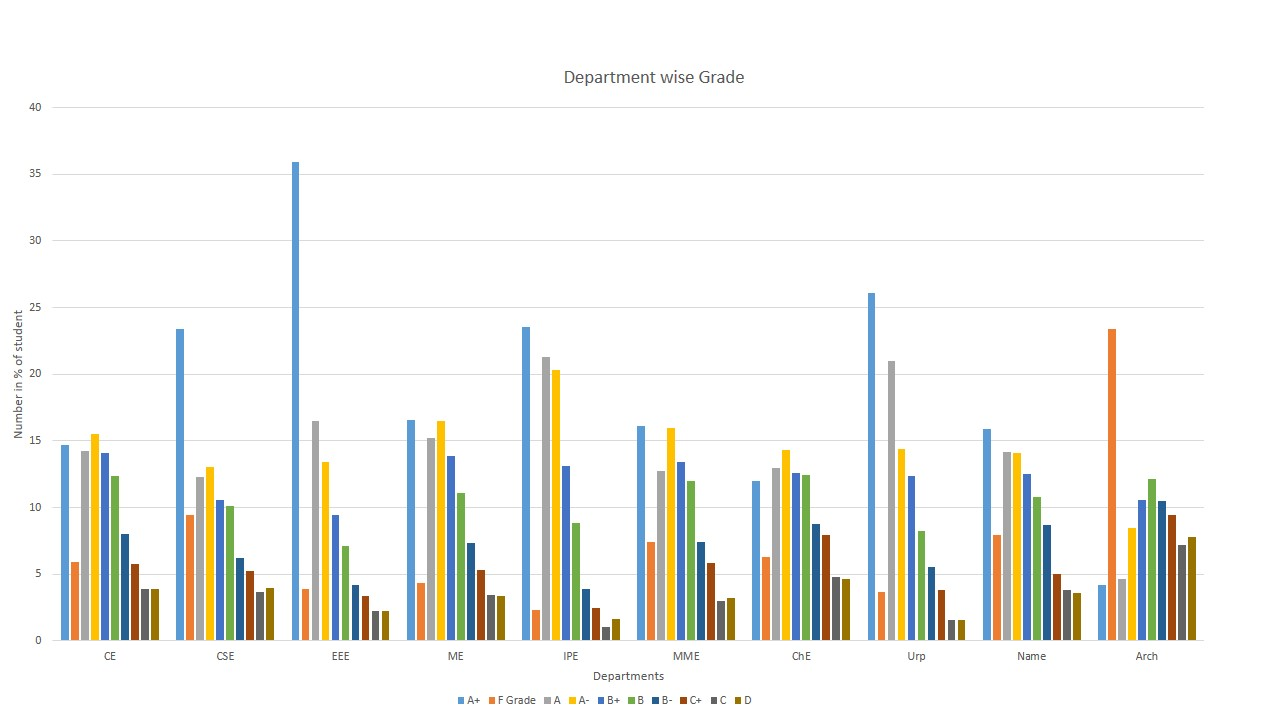
\includegraphics[width=\linewidth]{Figures/deptgrade.jpg}
  \decoRule
  \caption[Different Grades for Dept]{Different Grades for Dept}
  \label{fig:Different Grades for Dept}
\end{figure}

Figure \ref{fig:Different Grades for Dept} shows the frequency of different letter grades for different department.
For example students of EEE department get A+ more than other grades. On the other hand students of Architecture department get most percentage of F grade among other grades. 


\begin{figure}[H]
   \centering
  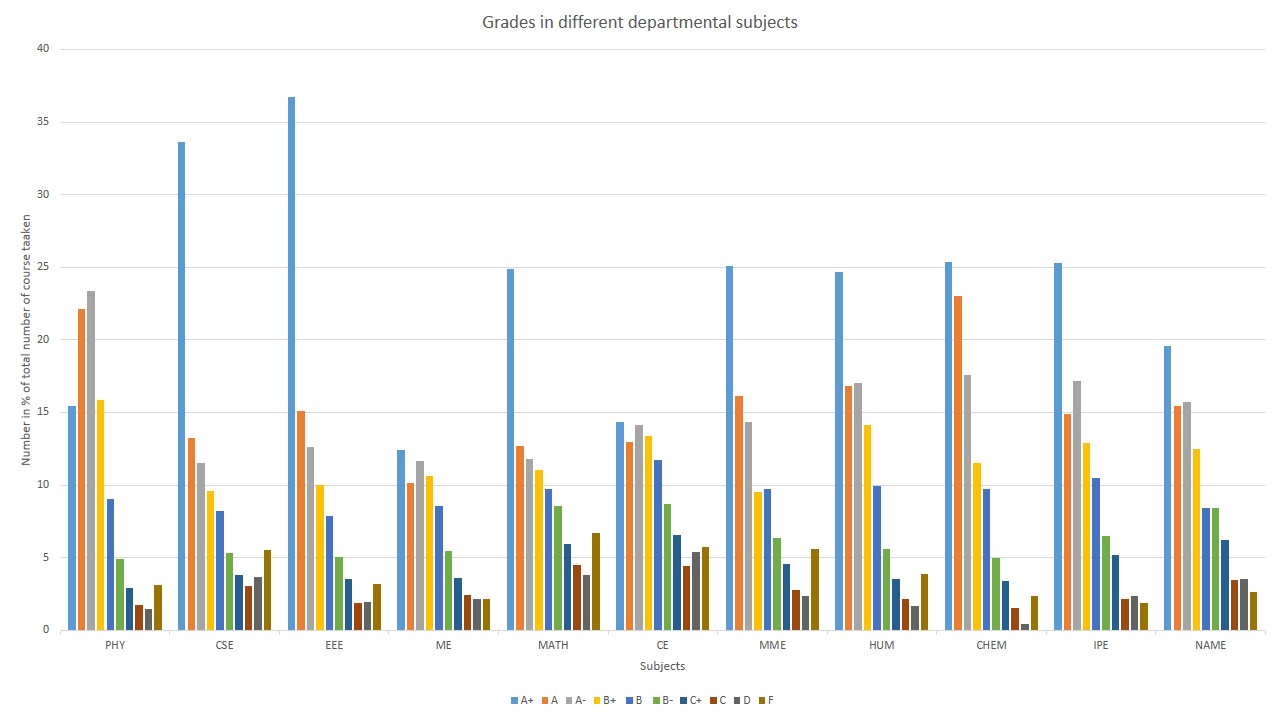
\includegraphics[width=\linewidth]{Figures/depresult.jpg}
  \decoRule
  \caption[Different Grades for Subjects]{Different Grades for Subjects}
  \label{fig:Different Grades for Subjects}
\end{figure}


Figure \ref{fig:Different Grades for Subjects} shows the frequency of grades in different departmental subjects.
As we can see students get most A+ in EEE subjects and get most F grade in MATH subjects.
